%%%  \chapter{introduction}


%%%%%%%%%%%%%%%%%%%%%%%%%%%%%%%%%%%%%%%%%%%%%%%%%%%%

%%%%%%%%%%%%%%%%%%%%%%%%%%%%%%%%%%%%%%%%%%%%%%%%%%%%

\section{ProtoDUNE-SP in the context of DUNE/LBNF}

ProtoDUNE-SP is the single-phase DUNE Far Detector prototype that will be constructed and operated at the CERN Neutrino Platform (NP) starting in 2017. It was proposed to the CERN SPSC in June 2015 (SPSC-P-351), and following positive recommendations by SPSC and the CERN Research Board in December 2015, was approved at CERN as experiment NP-04 (ProtoDUNE). The Fermilab Director and the CERN Director of Research and Scientific Computing signed a Memorandum of Understanding (MoU) for this experiment in December 2015 that is initially valid until December 2022, % in the first instance, 
and may be extended by mutual agreement. 

%ProtoDUNE-SP, a significant experiment in its own right, will have a total liquid argon (LAr) mass of \kt{0.77} and represents the largest monolithic single-phase LArTPC detector to be built to date. %so far. 
%The CERN Neutrino Platform, in an extension to the EHN1 hall in the North Area, will provide a new dedicated charged-particle test beamline. ProtoDUNE SP aims to take its first beam data before the LHC long shutdown (LS2) at the end of 2018.

%ProtoDUNE-SP is a crucial part of the DUNE effort towards the construction of the first DUNE \ktadj{10} far detector module, that will have a total LAr mass of about \kt{17}. It will prototype the designs of most of the DUNE far detector components at a 1:1 scale and with an extrapolation of about 1:20 in total mass size, very similar to the scaling factor adopted in the past by ICARUS from the 10-m$^3$ prototype to the T600 detector (two half-modules of about 375 t total LAr mass each).

ProtoDUNE-SP, a crucial part of the DUNE effort towards the construction of the first DUNE \ktadj{10} fiducial mass far detector module (17\,kt total LAr mass), is a significant experiment in its own right. ProtoDUNE-SP, with a total liquid argon (LAr) mass of 0.77\,kt, represents the largest monolithic single-phase LArTPC detector to be built to date. %so far. 
It will be housed in an extension to the EHN1 hall in the North Area, where the CERN NP will provide a new dedicated charged-particle test beamline. ProtoDUNE-SP aims to take its first beam data before the LHC long shutdown (LS2) at the end of 2018.

ProtoDUNE-SP will prototype the designs of most of the single-phase (SP) DUNE far detector components at a 1:1 scale, with an extrapolation of about 1:20 in total mass size,. \fixme{mass and size?} This is very similar to the scaling factor adopted %in the past 
by ICARUS; its T600 detector, split into two half-modules of about 375\,t total LAr mass each, was preceded by a 10-m$^3$ prototype.


The SP detector elements, consisting of the time projection chamber (TPC), the cold electronics (CE), and the Photon Detection System (PDS), are housed in a cryostat that contains the liquid argon target material. The cryostat, a free-standing steel-framed vessel with an insulated double-membrane system, is based on the technology used for liquefied natural gas (LNG) storage and transport. % ships. 
%A cryogenics system keeps the LAr at a stable temperature of about 89\,K through a process of recovering evaporated argon, recondensing it and returning it to the cryostat via a closed loop for forced recirculation of the liquid through the O$_2$ and H$_2$O filtration system that ensures the required LAr purity. 
A cryogenics system maintains the LAr at a stable temperature of about 89\,K and at the required purity level through a closed-loop process that recovers the evaporated argon, recondenses and filters it, and returns it to the cryostat. 


The TPC, illustrated in Figure~\ref{protodune-sp-tpc-touramanis}, includes the Anode Plane Assemblies (APA), the Cathode Plane Assemblies (CPA), and the field cage (FC), all components identical in design to those for the Far Detector. It consists of two arrays of three 6-m$\times$2.3-m wire-wrapped APAs at the opposite sides of the central CPA. Each APA is made of three parallel planes of wires (4.5 mm pitch, 2,560 wires) 
\fixme{the details in parentheses seem unnecessary (and distracting) here.}
oriented at different angles with respect to each other. The CPA is held at $-$180\,kV providing the 500-V/cm drift field in the 3.6-m drift regions between the CPA and APAs. % (also identical to the Far Detector configuration). 
Uniformity of the electric field is guaranteed by the FC that delimits the volumes between CPA and APA planes.

\begin{cdrfigure}[ProtoDUNE-SP TPC]{protodune-sp-tpc-touramanis}{ProtoDUNE-SP TPC}
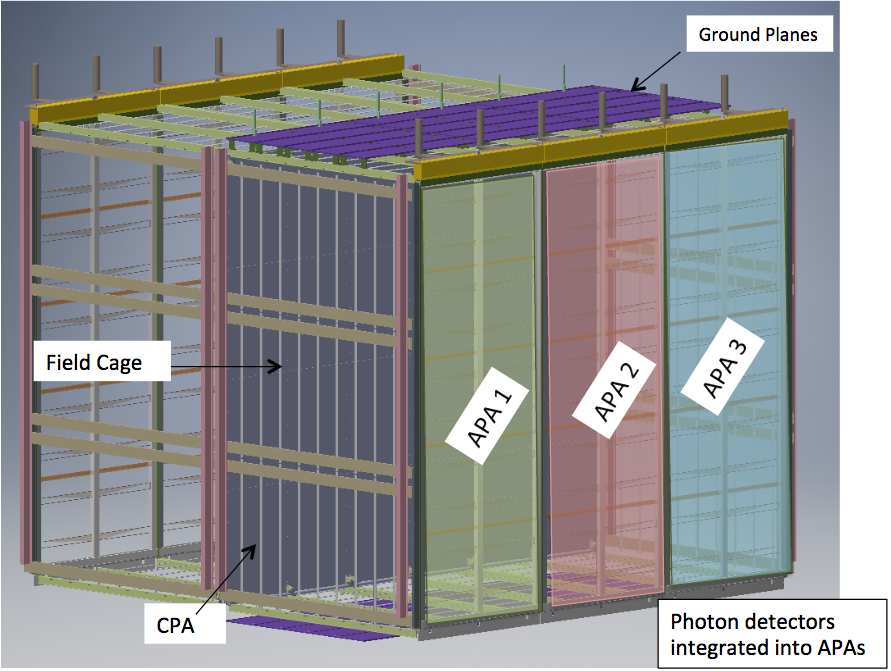
\includegraphics[width=0.9\textwidth]{protodune-sp-tpc-touramanis}
\end{cdrfigure}

The CE, mounted onto the APA frame and immersed in LAr, amplifies and continuously digitizes the induced waveforms on the sense wires at several MHz, and transmits these data to the Data Acquisition system (DAQ). The data are then transmitted through the buffer to disk, then to the central CERN Tier-0 Computing Center and finally to other partner sites for processing and analysis.  

The current PDS reference design uses a thin radiator coated with a wavelength-shifting layer of tetraphenyl-butadiene (TPB) that converts incoming VUV (128 nm) %Ar 
scintillation photons to longer wavelength photons, in the visible blue range. 
\fixme{previous sentence would read better with `light' rather than `photons'} The radiator is placed in front of a doped acrylic bar 200 cm long and 7.6 cm wide. Half of the converted photons will be emitted into the bar. A fraction of the wavelength-shifted optical photons are then internally reflected to the bar's end where they are detected by silicon photomultipliers (SiPMs).
The APA frame is designed with ten bays into which PDS modules (coated bars) can be inserted. The bars are inserted into the frames after the TPC wires have been strung, allowing final assembly at the integration area at the CERN NP prior to installation inside the cryostat. 

%After completion of the detector mounting, LAr filling and commissioning of the prototype detector, 
Once the prototype detector is commissioned, the charged-particle beam test will provide critical calibration measurements necessary for precise calorimetry as well as invaluable data sets for optimizing the event reconstruction algorithms -- i.e., for finding interaction vertices and for particle identification -- and ultimately for quantifying and reducing systematic uncertainties. These measurements are expected to significantly improve the physics reach of the DUNE experiment.

Other important goals for ProtoDUNE-SP include validation of the membrane cryostat technology and associated cryogenics, and of the networking and computing infrastructure that will handle the data and simulated data sets.
%ProtoDUNE-SP is thus an indispensable step to validate and benchmark the DUNE far detector engineering, to provide a well characterized charged-particle beam data set and to validate and test associated infrastructure requirements.  Given its technical challenges, its importance to the DUNE experiment and the timeframe in which it must operate, ProtoDUNE-SP requires a strong organizational structure and a collaborative effort from most of the DUNE Collaboration including US National Laboratories and University groups, CERN and international partners in the EU and Latin America. 
The construction and operation of ProtoDUNE-SP are thus indispensable steps toward the first DUNE Far Detector module. ProtoDUNE-SP will allow the collaboration to validate and benchmark the far detector engineering, to validate and test associated infrastructure requirements, and to extend the physics reach of the experiment. 


%%%%%%%%%%%%%%%%%%%%%%%%%%%%%%%%%%%%%%%%%%%%%%%%%%%%
\section{Goals of ProtoDUNE-SP}


%The primary goal of the ProtoDUNE-SP test program at CERN is very clearly a twofold one: First,  to benchmark and, if found fully adequate, to endorse the main technical solutions for the DUNE far detector components, and secondly, to perform the measurements needed to understand and possibly quantify the systematic uncertainties that will affect the DUNE oscillation measurements. The latter goal anticipates physics outcomes relevant on their own.
The ProtoDUNE-SP test program at CERN has two very clear primary goals. First, it will benchmark the principal technical solutions for the DUNE SP far detector components and, if they are found to be fully adequate, to endorse them. Secondly, it will perform the measurements needed to understand, and quantify to the extent possible, the systematic uncertainties that will affect the DUNE oscillation measurements. This second goal anticipates physics outcomes that will be relevant independent of the Far Detector.

%The detector operation in real experimental conditions and for an extended run period will allow for a full characterization of all the components, from the membrane cryostat and the cooling and purification circuit, to the APA design and its read-out cold electronics layout and HV system, to the photon detection system and its read-out warm electronics.
Operating the detector in real experimental conditions and for an extended period will allow for a full characterization of the components, including the membrane cryostat and the cooling and purification circuit, the APA design and the layout of its cold read-out electronics, the HV system, and the PDS and its warm read-out electronics.

The use of a well defined test beam of charged particles of known type and incident  energy will significantly enhance the understanding of the ultimate performance of the LArTPC technology and boost the optimization of event reconstruction, particle identification (PID) algorithms and calorimetric energy measurements.  The beam measurements will serve both as a calibration data set to tune the Monte Carlo simulations and as a reference data set for the DUNE experiment. 

%%%%%%%%%%%%%%%%%%%%
\subsection{Physics}

\fixme{The separation of physics vs engr goals may not be quite right yet}

%Pion and proton beams from around one to a few GeV will be used primarily to study hadronic interaction mechanisms, secondary particle production and, at higher energies, shower reconstruction and energy calibration. Electrons will be used to benchmark and tune electron/photon separation algorithms, to study electromagnetic cascade processes and to calibrate electromagnetic showers at higher energies. Charged kaons produced in the tertiary beam line are rare but are copiously produced by the pion beam interactions inside the detector. These will be extremely useful to characterize kaon identification efficiency for proton decay sensitivity studies.  Samples of stopping muons with Michel electrons from muon decay (or without, in case of negative muon capture) will be used for energy calibrations in the low energy range of the SN neutrino events and for the development of charge-sign determination methods. 
Pion and proton beams in an energy range from about one to a few GeV will be used primarily to study hadronic interaction mechanisms and secondary particle production.  At higher energies, these beams will be used to study shower reconstruction and energy calibration. Electrons will be used to benchmark and tune electron/photon separation algorithms, to study electromagnetic cascade processes and to calibrate electromagnetic showers at higher energies. Charged kaons produced in the tertiary beamline are rare but are copiously produced by the pion beam interactions inside the detector. These will be extremely useful for characterizing kaon identification efficiency for proton decay sensitivity studies.  Samples of stopping muons with Michel electrons from muon decay (or without them, in the case of negative muon capture) will be used for energy calibrations in the low-energy range of the SN neutrino events and for the development of charge-sign determination methods. 

A cumulative ProtoDUNE-SP test-beam run period of eight weeks is assumed, but it depends on the extent of beamline sharing with other users at EHN1. The run will take place prior to the long shutdown of the LHC in late 2018 (LS2). 

%During no-beam time cosmic data will be acquired. A dedicated external trigger system consisting of arrays of scintillator paddles, suitably positioned and arranged in coincidence trigger logic, will select specific classes of cosmic muon events. Dedicated runs, e.g. long muon tracks crossing the entire detector at large zenith angles allow for an overall test of the detector performance and the DAQ. Muons stopping inside the LAr volume and the accumulation of accurate Michel electron spectra may serve for energy calibration purposes in the low-energy range.
ProtoDUNE-SP will acquire cosmic data during periods with no beam. A dedicated external trigger system consisting of arrays of scintillator paddles, suitably positioned and arranged in \textit{coincidence} trigger logic, 
will select specific classes of cosmic muon events. Dedicated runs, e.g., runs looking for long muon tracks crossing the entire detector at large zenith angles, allow for an overall test of the detector performance and the DAQ. Runs looking for muons stopping inside the LAr volume and the accumulation of accurate Michel electron spectra may be useful for energy calibration purposes in the low-energy range.

%It is important to note that, besides calibration purposes and detector performance characterization, the unprecedented event reconstruction capability of the LArTPC technology combined with the large active volume of the ProtoDUNE-SP detector exposed to the CERN charged-particle beams open the way to a truly rich program of new physics investigations on particle interaction processes. The LArTPC features simultaneously precise tracking (3D imaging detector) and accurate measurement of energy deposited (homogeneous calorimeter). The large size of the active volume in ProtoDUNE allows for good containment of the hadronic and electromagnetic interaction products in the few GeV range. No other detector ever had all these features combined in one. 

It is important to note that ProtoDUNE-SP offers much beyond calibration  and detector performance characterization.  The LArTPC simultaneously features precise 3D tracking and accurate measurement of energy deposited. Its large active volume allows for good containment of the hadronic and electromagnetic interaction products in the few GeV range. These capabilities have never before been combined in one detector.  The unprecedented event reconstruction capability combined with the exposure of the detector's large active volume to the CERN charged-particle beams open the way to a truly rich program of new physics investigations into particle interaction processes. 


% Hadroninc ($\pi$, K and $p$) interactions on an Ar target around 1 GeV produce low multiplicity final states rather than "hadron showers",  and 1 GeV-electrons  (critical energy $\simeq 30$ MeV in Ar) produce low-populated cascades, with only a few tens of secondary energetic electrons(positrons). "TPC/imaging-aided calorimetric measurements" in this energy range may allow to investigate energy deposition mechanisms and reconstruction methods where the usual hadronic and el.m. shower concepts and features are not well defined or cannot be applied.Calorimetric measurements of the energy deposited can be accomplished,  whenever possible, for each individual secondary particle/track thanks to the imaging capabilities of this type of detector.In particular, the determination of the el.m. content in hadron initiated cascades, $\pi^0$ multiplicity and the energy fraction carried as a function of primary hadron incident energy will be of interest.


 Hadroninc ($\pi$, K and $p$) interactions on an Ar target around one GeV produce low-multiplicity final states rather than ``hadron showers,'' 
 and 1-GeV electrons  (with critical energy $\simeq 30$ MeV in Ar) produce low-populated cascades, with only a few tens of secondary energetic electrons (positrons). \fixme{I don't see relationship between this sentence and next. Maybe need a ``therefore'' in next sentence?}
``TPC/imaging-aided calorimetric measurements'' in this energy range may allow investigation of 
energy deposition mechanisms and reconstruction methods where the usual hadronic and electromagnetic shower concepts and features are either not well defined or cannot be applied.
Calorimetric measurements of the energy deposited can be accomplished,  whenever possible, for each individual secondary particle/track thanks to the imaging capabilities of this type of detector.
\fixme{the `wherever possible' makes the sentence meaningless; please clarify}
In particular, the determination of the electromagnetic  content in hadron-initiated cascades, $\pi^0$ multiplicity, and the energy fraction carried as a function of primary hadron incident energy will be of interest.

\fixme{This whole last paragraph is somehow not gripping me; could it be clarified and then maybe put above the previous paragraph (which would make a better conclusion.}
%In conclusion, test beam data will be essential for a rich physics program with ProtoDUNE at the CERN NP.


%%%%%%%%%%%%%%%%%%%%
\subsection{Detector engineering validation}  % was previously sec 2.4 in sciencetech file

One of the primary goals of the ProtoDUNE-SP experiment is to validate the engineering design of the elements proposed for the 10 kt DUNE single-phase detector. ProtoDUNE-SP is designed so that it will provide information on the actual far detector performance in as close a possible a configuration to the actual far detector layout as possible given the practical considerations imposed by time, space, and cost. To achieve this the cold components are wherever possible identical to the components proposed for the far detector. 

As an example the APA modules are full-scale pre-production modules for the far detector. The full-scale APA modules have 20 front end readout board instrumenting each and 10 integrated photon detector paddles. The ground connections between the electronics, the APA mechanical structure, the photon detectors, and the detector support structure will be as proposed for DUNE SP detector. ProtoDUNE-SP is instrumented with three APAs along each wall which will test that there is no cross talk between the middle APA and the neighboring ones. However, there are some practical limitations which required compromise in the ProtoDUNE-SP design. The far detector is designed with a 12 m high TPC based on a two APA high layout where the bottom APA is hung from the top. Given the space available and generally the cost of the cryogenic infrastructure it is not practical to have a 12 m high test experiment. For these reasons ProtoDUNE-SP is designed with a single APA high TPC. The collaboration will test separately the mechanical process of installing the two APA detector configuration along with the related cabling.

The readout electronics is designed based on the far detector cryogenic front end pre-amp/shaper chip and ADC.  The dedicated ASIC for serializing the data and providing a 1GB/s link is not yet available so an FPGA emulating its functionality will be used and is mounted on a dedicated mezzanine board. It should be pointed out that all the analog components, the conversion to digital and the grounding/power distribution for the final electronics can be tested in this configuration. 

ProtoDUNE-SP will be the largest experiment to take data with the cold electronics allowing high statistic detailed studies of the performance. In the event further optimization of the ASICs are required based on the ProtoDUNE-SP findings, this can be implemented before production start in 2020. As there is no charge amplification in the liquid in the Single-Phase detector, the electronics must be extremely sensitive which makes the grounding and shielding critical. The ProtDUNE-SP experiment is designed to be as close to the far detector grounding as practical. The building ground in ENH1 with all the rebar in the concrete floor interconnected and then this network connected to the building ground bus should provide a fairly good ground for ProtoDUNE-SP. The cryostat itself is isolated from the building ground and all the mechanical/electrical connections have dielectric breaks. At the far site the detector is a mile underground in a very dry mine so one expects better isolation from the environment, but the ProtoDUNE-SP will test the ground isolation and shielding under conservative conditions.

The field cage and cathode planes are full-scale prototypes of the final far detector elements. As the ProtoDUNE-SP detector is designed with full-scale field cages the maximum drift distance and corresponding high voltage will be the same as planned for the far detector. This allows ProtoDUNE-SP to use the same high voltage feed thru as DUNE-SP and the drift field configuration that is planned for the far detector. The cryostat dimensions are selected to be the same as the Dual-Phase cryostat in order to only need to design one cryostat and cryogenic system. In order to fit in the cryostat the wall to cathode plane distance is slightly smaller than in the far detector making this setup a conservative test of the HV design. The ground planes above and below the detector make the actual mechanical geometry inside the cryostat on the top and bottom irrelevant for issues related to high voltage. This preserves the freedom to tailor the far detector cryogenics system as needed to optimize the purification without compromising the validity of the ProtoDUNE-SP test. 

Testing these components under nominal operating conditions is extremely important as this is the first instance of LArTPCs operating with a resistive cathode or the field cage construction with metal profiles and fiberglass I-beam support. In the event ProtoDUNE-SP wishes a second run with a shorter drift distance in order to reduce the effects of space charge the FC can be shortened to 2.5 m maximum drift distance.

ProtoDUNE-SP offers a unique platform to validate and possibly optimize the cryogenic design for DUNE. The DUNE 35-t prototype was the first membrane cryostat to achieve high purity operation, but it was limited to roughly 3 ms $e^-lifetime$. This is substantially worse than the MicroBooNE experiment's  $\sim$10 ms or the lifetimes seen at ICARUS at the end of its last run. 

There are several possible causes for a shorter electron lifetime.  A third of the 35-t cryostat roof is covered with a hatch that is not insulated but designed with radiation shields. As the dominant source of contamination is the transfer of impurities in the gas ullage to the liquid, the gas circulation in the ullage and the impact of the hatch are important factors in the cryostat/cryogenics design. The purity monitors inside the 35-t cryostat also indicated that the liquid was not well mixed with substantially higher purity at the bottom of the cryostat indicating that the liquid feed and temperature need to be optimized.  

The ProtoDUNE-SP cryostat design does not have a hatch for the detector installation instead a temporary construction opening (TCO) is used (similar to the Dual-Phase cryostat). The Single-Phase detector moved to this option after the difficulties encountered in the mechanical design of the hatch for the 1x1x3 cryostat and based on the recommendations from the cryostat design team.  This will also eliminate one potential source of contamination to the liquid argon. It should be pointed out that with a 3 ms lifetime and a 2.25 ms maximum drift time roughly half the charge generated near the cathode is lost before it reaches the anode. Efforts to improve the electron lifetime will improve the detector performance.  Cryogenic design improvements are that the Proto-DUNE SP detector will not have a hatch in the ullage, all cryostat penetrations will be designed with gas purge to prevent contaminates from migrating from warm surfaces to the ullage volume, and the cryostat/cryogenic system will be modeled to understand the liquid and gas flows inside the cryostat. ProtoDUNE-SP will provide an excellent test bed to prove the cryogenic design for DUNE. 

The installation process has many similarities to the far detector installation but also many differences. Both installation plans now call for inserting the equipment through a TCO. ProtoDUNE-SP will prototype the tooling and procedures for transporting an APA and transferring to to a suspended rail system. Similarly the assembly and transport of the cathode planes and top/bottom field cages will be developed. What will not be tested is the hanging of one APA from the other and the difference in moving a 12 m stack instead of one 6 m module. Likewise the CPA is only 6 m tall instead of 12 m. One major change in the installation was forced by the need to install the end walls with the TCO closure and the beam interface. Due to the tight space inside the cryostat the rail structure on which the detector is hung will most likely be different for the final detector. However the experience in installing the ProtoDUNE-SP detector will be invaluable in planning the DUNE far detector installation. 

Finally one significant difference between the ProtoDUNE-SP detector and the single-phase far detector is the integration of the test beam. This requires a penetration into the cryostat and a liquid argon displacement plug bridging the gap between the membrane cryostat wall and the detector field cage. As this element bridges the high voltage careful design is required. To insure that the displacement plug does not compromise the ProtoDUNE-SP operation a dedicated HV test at FNAL is planned which will test the final beam plug in the exact field configuration planned for ProtoDUNE-SP.

%%%%%%%%%%%%%%%%%%%%%%%%%%%%%%%%%%%%%%%%%%%%%%
\section{Run Plan}
\label{sec:runplan}

\fixme{May need some intro/transition content here since this section was just moved in from a different part of the document}

Beam simulations show that the hadron rates at 
energies below 1~GeV/c are low. Moreover, low-energy beams are more
subject to degradation by materials in the
beamline.  The optimization of the run plan factors in the beam composition and particle rates of the H4 beamline, and 
also particle interaction topologies in the ProtoDUNE-SP detector. Full FLUKA~%\cite{fluka05,Fluka15}
simulations of particle transport in the ProtoDUNE-SP detector, including the
beam window, have been performed.
% The physics requirement \fixme{that the beam must satisfy overall? Anne} is %the possibility 
% to enable measurement of
% stopping particles and  interactions at both high and low energies.    
%
At a beam momentum of 1~GeV/c, 35\% of protons are stopped before reaching the active TPC region, while the percentage reduces to 0.5\% at 2~GeV/c.  The kinetic energy distributions of protons and pions at the entrance point of the TPC for different beam momenta are shown in Figure~\ref{fig:pandpiint}. 
%The residual energy at the interaction point can be reconstructed by measuring the energy deposited along the proton track.
The fraction of stopping $\pi$'s for one $\pi$
produced at the secondary target is 3\% at $p=0.4$~GeV/c and decreases to 1.3\% at $p=0.7$~GeV/c.
%Having a $\pi$ beam at 0.7~GeV/c still allows 
%measurement of pion interactions down to few tens of MeV with good
%statistics. In a 1-GeV/c beam, the low-energy interactions are %still
%present, albeit at a %with 
%lower rate, as shown in Figure~\ref{fig:pandpiint}.
%
The long distance (37~m) between the secondary target and the front of the LAr cryostat has a significant impact on the pion and kaon rates in the TPC. Due to pion lifetime, many of the  low-energy pions produced at the secondary target decay in the beam pipe before reaching the cryostat. The situation is even more significant for kaons; most kaons below 2~Gev/c do not make it to the cryostat.
Consequently we will not operate the H4 beamline much below 1~GeV/c in the hadron mode.
For electrons, we would want the beam momentum to go as low as possible to study the topology of very low-energy electron-initiated 
showers.
\begin{cdrfigure}[Energy at interaction]{pandpiint}{Kinetic energy of
    particles at the point of interaction in the ProtoDUNE-SP active
    volume, for different beam momenta. Histograms are normalized to one particle injected in the
    beamline acceptance. FLUKA simulations include the beam window
    materials, beams are considered as monochromatic and
    parallel. Left: protons, Right: pions.}
  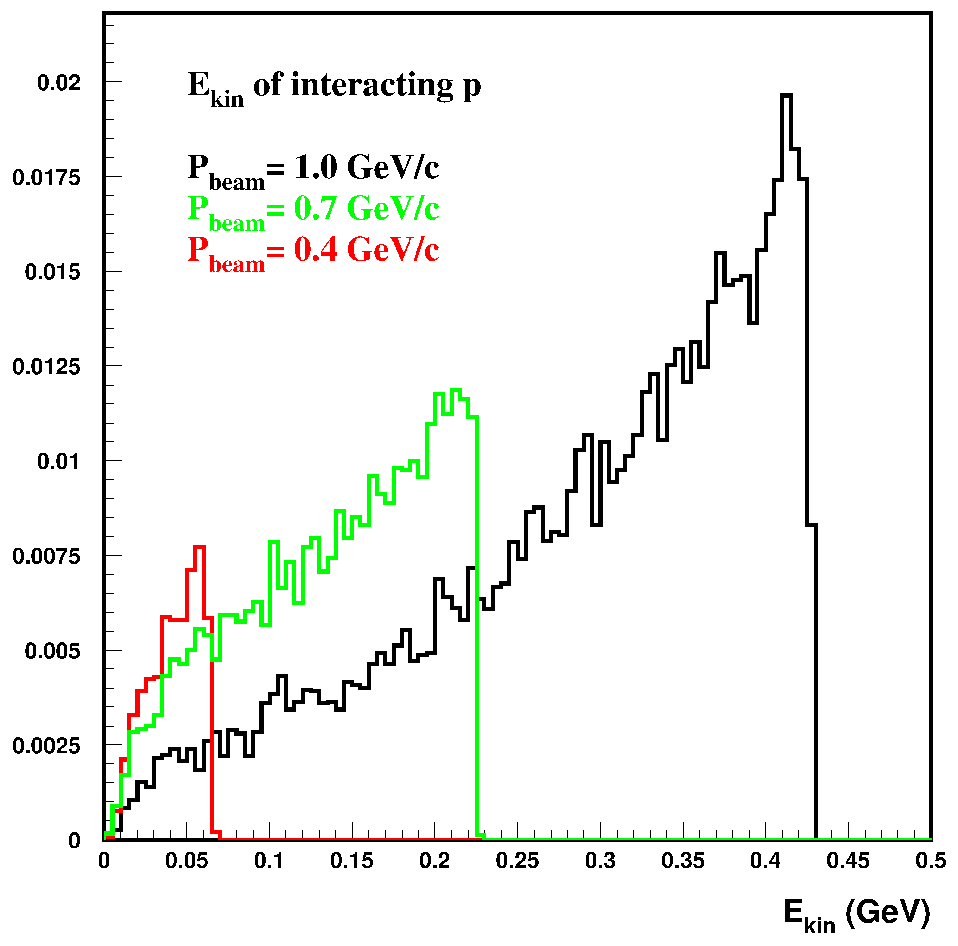
\includegraphics[width=0.49\textwidth]{pvarie_intene.pdf}
  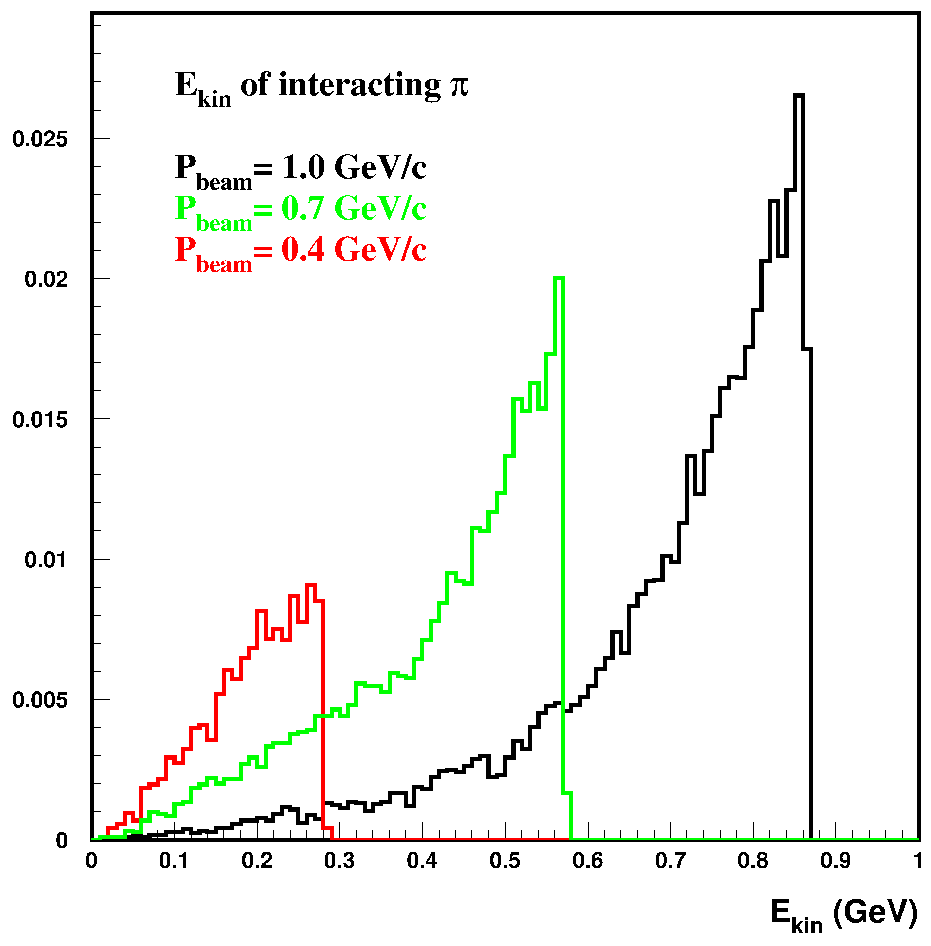
\includegraphics[width=0.49\textwidth]{pivarie_intene.pdf}
\end{cdrfigure}
%% end of   part that can go either here or in the run plan 

To formulate a preliminary run plan, we assume the hadron beam spectrum and rates are as given in Tables~\ref{tab:beampartcomp} and~\ref{tab:beampartrates}.   For the purpose of estimating the sample composition and beam time request, the following assumptions are used:
\begin{itemize}
\item { Trigger rate = 25~Hz}
\item { Two 4.8 sec spills per SPS Super Cycle }
\item { SPS Super Cycle = 48 sec}
\item { $10^6$ ($10^4$) secondary particles on target per spill for hadron (electron) beam}
\item { Particle ID trigger for electrons from 0.5 to 7 GeV/c}
\item { Trigger rate for electron in hadron beam is prescaled to 0.5~Hz}
\item { Data collection efficiency = 50\%}
\end{itemize}
We plan to run the H4 beamline in two modes: the first configuration is optimized for the production of hadrons and the second configuration is optimized for the production of high purity electrons. Even in the hadron mode, the beam is still dominated by electrons, especially for low beam momenta. However, the electrons in the hadron beam are not particularly ``clean'' due to the amount of materials in the beamline from the particle identification (PID) instrumentations .  The proposal is to heavily prescale the electron events using PID (e.g. Threshold Cherenkov counters) trigger while running in hadron mode. The PID systems that contribute significantly to the material budget will be removed when we reconfigure the beamline for electron beam.  We are exploring various run plan scenarios. One of the scenarios is shown in Tables~\ref{tab:HadRunPlan} and ~\ref{tab:ElecRunPlan}. Tables with similar values are expected for the negative beam sample. 
\begin{cdrtable}[Preliminary run plan for ProtoDUNE-SP hadron beam]{ccccccccc}{HadRunPlan}{A preliminary run plan for ProtoDUNE-SP hadron beam. The expected sample (positive beam) as a function of momentum is shown. }
P & \# of  &\# of $e^+$ & \# of $K^+$ & \# of $\mu^+$ & \# of $p$ & \# of $\pi^+$ & Total \# & Beam Time \\ 
(GeV/c) & Spills  & &  &  &  &  & of Events & (days) \\ \toprowrule
1 & 70K & 84K & $\approx$ 0 & 13K  & 672K & 504K & 1.3M & 19 days\\ \colhline
2 & 20K & 24K & 8K & 21K     & 336K & 480K & 0.9M &5.6 days\\ \colhline
3 & 12K & 14K & 14K  & 14K   & 163K & 516K  & 720K & 3.3 days\\ \colhline
4 & 10K & 12K & 23K & 15K    & 90K  & 460K & 600K & 2.8 days\\ \colhline
5 & 10K & 12K  & 25K  & 6K   & 81K  & 475K & 600K & 2.8 days\\ \colhline
6 & 10K & 12K & 34K  & 5K    & 82K  & 468K & 600K & 2.8 days\\ \colhline
7 & 10K & 12K & 34K & 7K     & 80K  & 467K & 600K & 2.8 days\\ \toprowrule
Total & 142K & 170K & 132K & 81K & 1.5M & 3.4M & 5.3M & 39 days\\
\end{cdrtable}
\begin{cdrtable}[Preliminary run plan for ProtoDUNE-SP electron beam]{cccc}{ElecRunPlan}{A preliminary run plan for ProtoDUNE-SP electron beam. The expected sample for positive beam configuration is shown. }
Momentum Bins & \# of Spills per Bin & \# $e^+$ per Bin & Beam Time per Bin \\ 
(GeV/c) & & & (days) \\ \toprowrule
0.5, 06, 0.7, 0.8, 0.9, 1, 2, 3, 4, 5, 6, 7 & 5000 & 300K & 1.4 \\
\end{cdrtable}

Based on the current information available, the total estimated beam time needed to carry out the physics program in this proposal with the assumptions stated earlier is on the order of 16 weeks.
 
 



